% We do not want to have screen shots of the celebrity puzzle in this section:
\clearpage
\section{Proving Deadlock Freeness}
\label{tut_location_access_controller}

\tick{\textbf{Goals:} In this section, we will take a closer look at a few more complex proofs. Here we use the model of a location access controller. The goal is to develop the proofs that ensure there are no deadlocks present in the initial model and in the first refinement.}

\info{This example has been taken from the Event-B book (\ref{abrial_2010}) and is quite sophisticated.  In this section, we are dealing with a subset of the complete model.  We encourage readers to consult the example in the book.}

%\info {First of all you need to download the following \file{Doors.zip}{Location Access Controller problem}.}

Through the model used in this section, we study a complete system and mention the proof rules of formal development. This system's job is to control the access of certain people to different locations of a site. The system is thus based on whether a person has (or does not have) access to a particular location.

Before describing the initial model, import the archive file \file{Doors.zip}{Doors.zip} that contains the model. To do this, select  \textsf{File $\rangle$ Import $\rangle$ General $\rangle$ Existing Project into Workspace}. Then select the according archive file and click on \textsf{Finish}. It will take Rodin a few seconds to extract and load all the files.

\subsection{Deadlock Freeness of initial model}
\label{deadlock}
\label{tut_initial_model}

%Besides we introduce:

%\begin{itemize}
%	\item The two carrier sets of persons, P, and locations, L
%	\item The constant authorisation, \textbf{aut}, representing a relation between P and L, actually where people are allowed to go %(Axiom 1).
%	\item The variable, \textbf{sit}, which denote where a person is, \textbf{sit} is a function from P to L.
%\end{itemize} 
 
%Moreover, we introduce a special constant “location”, named \textbf{outside}. Everyone is authorized to be in outside (Axiom 3) and a %person cannot be in two locations at a time. However every person, which is in a certain location, is authorized to be there.

%Initially, everyone is outside as indicated in event \textsf{INITIALISATION}.
%The other event \textsf{PASS} of that model has to aim to change the location of a person.
%We call the proof of deadlock freeness through this tutorial the proof justifying that someone can always change location.

Let us look at the initial model which consists of the context \texttt{doors\_ctx1} and the machine \texttt{doors\_0}. There are two carrier sets in the model context. One is for people ($P$) and the other is for locations ($L$). There is a location called outside ($outside$) and a relation ($aut$) which defines the places that people are allowed to go. Everyone is permitted to go outside. The model machine has one event, \textsf{pass}, which changes the location of a person and one variable, $sit$, which denotes where a person is located. 


Looking through the initial model, you will see that everything already has been proved (for the initial model and initial contexts). This is true, but Rodin has not yet proved that the model is deadlock free yet, so we will have to prove this ourselves. A model is considered to be deadlocked if the system reaches a state where there are no outgoing transitions. The objective of this section is to develop proofs for deadlock freeness for the initial model and for the first refinement. 

Consider the event \textsf{pass} from the initial model:

\pencil{
\begin{description}
\EVENTS
	\EVT {pass}
		\begin{description}
		\AnyPrm
			\begin{description}
			\ItemX{ p }
			\ItemX{ l }
			\end{description}
		\WhereGrd
			\begin{description}
			\nItemX{ grd11 }{ p \mapsto  l \in  aut }
			\nItemX{ grd12 }{ sit(p) \neq  l }
			\end{description}
		\ThenAct
			\begin{description}
			\nItemX{ act11 }{ sit(p) :=  l }
			\end{description}
		\EndAct
		\end{description}
\END
\end{description}
}

\index{deadlock}
Since the initial model has only one event (\textsf{pass}), the system might deadlock when both guards of the event (\textsf{grd11} and \textsf{grd12}) are false.
In this case, to prove that no deadlocks can occur requires proving that someone can always change room. We must therefore prove that the two guards are always true. 
To do this, add a new derived invariant (a theorem) to \texttt{doors\_0} called \textsf{DLF} (click once on the label \texttt{not theorem} to make it switch to \texttt{theorem})
  and change the predicate so that it is the conjunction of the two guards.
The difference between a ``normal'' invariant and one that is marked as theorem is that you must prove that a theorem is always valid when the previously listed invariants are valid. Then we don't need to prove that an event preserves the invariant marked as theorem because we can conclude this logically when it already preserves the other invariants.

\pencil{
\begin{description}
\INVARIANTS
	\begin{description}
		\nItemX{ DLF }{ \fbox{theorem} ~ \exists p, l\qdot (p \mapsto  l \in  aut \land  sit(p) \neq  l) }
	\end{description}
\end{description}
}

\warning{ Make sure that when you add your DLF invariant, you add it after the other two invariants in \textsf{doors\_0}. The auto prover uses these invariants to prove that the DLF invariant is well defined, and if they aren't in the right order, the proof obligation \textsf{DLF/WD} will not be discharged
}

\begin{rodin-plugin}{img/prob.png}{ProB}%
  You can also use ProB to search for deadlocks (after ensuring that ProR is installed).
  Right-click on the machine you want to check and start the animation with the
  ``Start Animation / Model Checking'' menu entry.
  After starting the animation, go to the Event View in the ProB perspective
  (see Figure \ref{fig_tut_prob_perspective}).
  There are two ways to search for deadlocks:
  \begin{itemize}
  \item Press the \texttt{Check} button and mark \texttt{Find Deadlocks}. Then start the model checking by pressing the button \texttt{Start consistency checking}.
    ProB then systematically ``executes'' all events and tries to find a state where no
    event is enabled.
  \item An alternative is to select \texttt{Deadlock Freedom Checking} after clicking
    on the triangle to the right of the \texttt{Check} button.
    ProB will then prompt you to input a predicate, but this is optional, so leave it blank. The difference with this alternative alternative is that ProB searches now for variable values
    where all the invariants are valid but none of the guards are valid.
  \end{itemize}
\end{rodin-plugin}

Save the machine. We see in the \textsf{Event-B Explorer View} that the auto-prover (\ref{auto_prover}) fails to prove the theorem \textsf{DLF/THM}.

\warning{If you cannot find the proof obligation \textsf{DLF/THM}, maybe you forgot to mark the invariant as a theorem by clicking once on the \texttt{not theorem} label next to the invariant.
  Another reason that you might not see the proof obligation \textsf{DLF/THM} is that you have forgotten to rename the invariant ``DLF''.}

Let us analyze whether this is an inconsistency in the model. Switch to the \texttt{Proving Perspective } and double click on the proof obligation \textsf{DLF/THM}.
\index{post-tactics}
In the Proof Control view, first disable the post-tactics (there is a small downward pointing arrow in the upper right hand corner above the toolbar (see Figure~\ref{fig_tut_10_post_tactics}).
Click on this arrow and make sure that the option \textsf{Enable post-tactic} is unchecked in the dropdown menu.)
We are turning off the post-tactics because we want to see the proof develop in its different stages.
Now select the root node in the \textsf{Prove Tree}, right-click on it and select \textsf{Prune}.
This removes any proof that might be already started by the auto-provers.
By doing this we want to assure that you have the same proof as in this tutorial.

\begin{figure}[!ht]
  \begin{center}
    	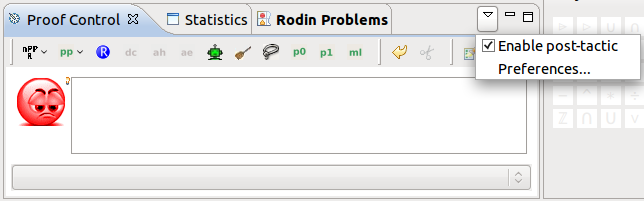
\includegraphics{img/tutorial/tut_10_post_tactics.png}
    \caption{Disabling the proof post-tactics in the Proof Controlling View}
    \label{fig_tut_10_post_tactics}
  \end{center}
\end{figure}

In order to succeed with the proof, we need a pair $p \mapsto l$ that is in $aut$ but not in $sit$.
Having a look the axioms, we find  \textsf{axm4} of \texttt{doors\_ctx1}, which states that 
  there is a location $l$ different from $outside$ where everyone is allowed to go:

\pencil{
\begin{description}
\AXIOMS
	\begin{description}
		\nItemX{ axm4 }{ \exists l\qdot l\in L\setminus \{ outside\}  \land  P\cprod \{ l\} \subseteq aut }
	\end{description}
\end{description}
}

So for every person $p$ in $P$, $p \mapsto l$ and $p \mapsto outside$ are in $aut$.
(In other words: every person is allowed to go to both the outside and a location $l$).
The basic idea of our proof is that a person is either already outside or at the location $l$. If someone is outside, they are allowed to move to $l$, and if they are not outside, they are allowed to move outside. \footnote{One could argue that this is too restrictive in the real world: After all, why do all people need authorisation for the \textit{same} location l?  But arguing about the realism of the example is out of the scope.}.

We assume that there is actually a person, so we need a set $P$ that is non-empty. 
This is automatically the case since carrier sets are always non-empty, but we need a person as an example for our further proof. 
Now add the hypothesis $\exists x \qdot x \in P$ by entering this predicate into the \textsf{Proof Control} text area and hitting the \icon{rodin/ah_prover.png} button.
In the \textsf{Proof Tree} view you can now see three new nodes have appeared that need to be proven:
\begin{itemize}
\item $\btrue$ is the trivial well-definedness condition. Click on \icon{rodin/auto_prover.png} button to verify it.
\item $\exists x\qdot x\in P$ is the hypothesis that we introduced. Click on the \icon{rodin/auto_prover.png} button to verify it.
\item $\exists p, l\qdot (p \mapsto  l \in  aut \land  sit(p) \neq  l)$ is the original goal
  but we can now use the introduced hypothesis in the proof. We will now continue with the proof of this goal.
\end{itemize}

Click on the existential quantifier of the new hypothesis $\exists x \cdot x \in P$
  (appearing in the \textsf{Selected Hypothesis} view) as demonstrated in Figure \ref{fig_tut_10_instantiate_x}.
The hypothesis disappears and is replaced by a new hypothesis $x \in P$. This is because the value of $x$ is automatically instantiated. This means that we can use $x$ from now on in our proof as an example for a person

\warning{If you hover over any red symbol for a short while, a menu will pop up, offering one or more transformations.  Make sure that you actually click on the symbol before the menu pops up because otherwise clicking will no longer have any effect.  If the menu has popped up before you managed to click on the symbol, you will have to click twice: the first click will discard the menu and the next click will actually perform the operation.}

We can prove an existential quantification by giving an example for the variables. First, we
  instantiate $p$ in the goal with the variable $x$ that we created: enter $x$ in the yellow box corresponding to $p$ 
  in the \textsf{Goal View} and click on the existential quantifier as shown in Figure \ref{fig_tut_10_instantiate_p}. 

\begin{figure}[!ht]
\begin{center}
	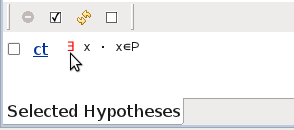
\includegraphics{img/tutorial/tut_10_instantiate_x.png}
	\caption{Click on the existential quantifier in order to ...}
	\label{fig_tut_10_instantiate_x}
\end{center}
\end{figure}

\begin{figure}[!ht]
\begin{center}
	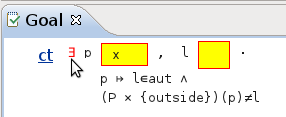
\includegraphics{img/tutorial/tut_10_instantiate_p.png}
	\caption{... instantiate it, in this case by substituting $x$.}
	\label{fig_tut_10_instantiate_p}
\end{center}
\end{figure}

% \warning{If the hypothesis does not appear immediately in the \textsf{Selected Hypothesis} view, reclick on the Auto Prover button until it does.}

The instantiation produces two new nodes in the \textsf{Proof Tree} view. The first goal is the trivial well-definedness condition $\btrue$ and
  can be easily discharged by pressing \icon{rodin/auto_prover.png}.
The remaining goal is $\exists l\qdot (x \mapsto  l \in  aut \land  sit(x) \neq l)$ is the result of replacing $p$ by $x$ in the old goal.
You can see the the current proof tree in Figure~\ref{fig_tut_10_proof_tree}. The node with the label \textsf{ah} refers to when we added the hypothesis, the node with the label \textsf{$\exists$ hyp} refers to when we instantiated $x$ from a hypothesis and the node with the label \textsf{$\exists$ goal} refers to when we instantiated $p$ in the goal.

\begin{figure}[!ht]
\begin{center}
	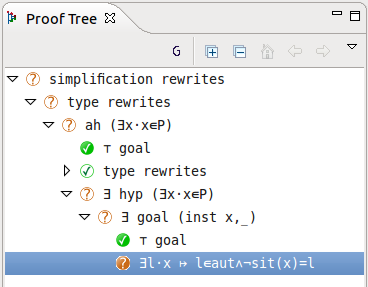
\includegraphics{img/tutorial/tut_10_proof_tree.png}
	\caption{The proof tree after instantiating $p$ with $x$.}
	\label{fig_tut_10_proof_tree}
\end{center}
\end{figure}

Now we need an example for the remaining variable $l$.
There are two situations we want to distinguish: The person $x$ could be outside or not.
To distinguish this, type $sit(x) = outside$ into the \textsf{Proof Control} view and click on the button \icon{rodin/dc_prover.png} (\textsf{dc} for distinguish case).
Again, you get three new goals.

\begin{itemize}
\item The first is the well-definedness condition of $sit(x) = outside$. $sit$ must be a function and $x$ is in its domain.
  This is easy to prove since $sit$ is a total function (\ref{relations}). Press the \icon{rodin/p1.png} button to verify it.
\item The second node has the original goal but $sit(x) = outside$ as a hypothesis.
\item The third node has the original goal but $\lnot sit(x) = outside$ as a hypothesis.
\end{itemize}

\warning{Note that the second and third node will appear identical in the proof tree.  You will only see the differences in the hypotheses by selecting the nodes.}

Let's continue with the case $sit(x)=outside$: When $x$ is outside, it can always go to the $l$ that is defined \textsf{axm4}.
To search for \textsf{axm4}, type $outside$ into the \textsf{Proof Control} text field and click the button \icon{rodin/sh_prover.png}. Add \textsf{axm4} ($\exists l\qdot l\in L\setminus\{outside\} \land P\cprod\{l\}\subseteq aut$) to the selected hypotheses. Now click on the red $\exists$ symbol in \textsf{axm4} (see Figure~\ref{fig_tut_10_search_hypotheses})
to instantiate $l$.
Now we have $l$ as an example for a location which is not outside and where everybody can go.
\begin{figure}[!ht]
  \begin{center}
    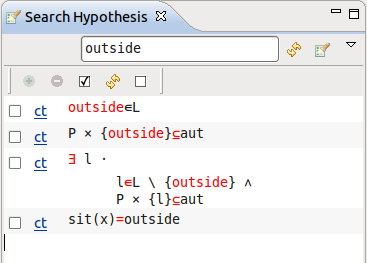
\includegraphics{img/tutorial/tut_10_search_hyp.png}
    \caption{Searching hypothesis for $outside$: The third one is \textsf{axm4}.}
    \label{fig_tut_10_search_hypotheses}
  \end{center}
\end{figure}
Our goal is still $\exists l\qdot x\mapsto l\in aut \land sit(x)\neq l$.
Note that the existential quantification introduces a new $l$ which does not (yet) have anything to do with
 the location $l$ where anybody can go.
Now type $l$ into the yellow box of the goal and press the $\exists$ symbol to state that we want to use our $l$ as
  an example for the $l$ in the existential quantification.
Again, we have the trivial goal $\btrue$ as well-definedness condition, so just press \icon{rodin/auto_prover.png} button to verify it.
The remaining goal should be $x\mapsto l\in aut \land sit(x)\neq l$.
This can be proven with the selected hypotheses $sit(x)=outside$, $l\in L\setminus\{outside\}$ and $P\cprod\{l\}\subseteq aut$. Press the \icon{rodin/auto_prover.png} button to verify this goal.

Now only second case of the case distinction remains. This is where $x$ is not outside ($sit(x)\neq outside$). In this case, $x$ can simply go outside.
Again the goal is $\exists l\qdot x\mapsto l\in aut \land sit(x)\neq l$. Type
$outside$ as an example for a location $l$ into the yellow box and press
the $\exists$ symbol.
Press  the \icon{rodin/auto_prover.png} button to discharge the trivial well-definedness condition $\btrue$.
The new goal should be $x \mapsto outside\in aut \land sit(x)\neq outside$.

To prove this we need to prove that $x$ has the right to go $outside$.
This is stated in the axiom $P \cprod\{outside\}\subseteq aut$.
Have a look at the \textsf{Search Hypothesis} view. This was also one of the results from the last search for $outside$.
(If you no longer see the results, repeat the search by entering $outside$ into the \textsf{Proof Control} and press the \icon{rodin/sh_prover.png} button.)
Select $P \cprod\{outside\}\subseteq aut$ (in Figure~\ref{fig_tut_10_search_hypotheses}, it's the second entry) and
  press the \icon{rodin/add.png} button to add it to your selected hypothesis. The auto-prover now has enough hypotheses, so simply click the \icon{rodin/auto_prover.png} button and
  the last goal of our theorem should be proven.

Here is the summary of the proof. Compare this with your final proof tree (as shown in 
Figure~\ref{fig_tut_10_final_proof_tree}).

\begin{tabular}{l}
  \hline
  added hypotheses: $\exists x\qdot x\in P$ \\
  \quad well-definedness condition $\btrue$: automatically proven\\
  \quad the hypotheses: automatically proven \\
  \quad instantiation of $x$ in the hypotheses $\exists x\qdot x\in P$\\
  \qquad using $x$ as an example for the $\exists p \ldots$ in the goal\\
  \quad\qquad well-definedness condition $\btrue$: automatically proven\\
  \quad\qquad case distinction $sit(x)=outside$ \\
  \qquad\qquad well-definedness condition
    ($sit$ is a function with $x$ in its domain): \\
  \qquad\qquad\qquad\qquad\qquad\qquad proven using the \textsf{p1} provers\\
  \qquad\qquad first case: instantiation of $l$ from axiom \textsf{axm4}\\
  \quad\qquad\qquad using $l$ as an example for the $\exists l \ldots$ in the goal\\
  \qquad\qquad\qquad well-definedness condition $\btrue$: automatically proven\\
  \qquad\qquad\qquad automatically proven\\
  \qquad\qquad second case: using $outside$ as an example for the $\exists l \ldots$ in the goal\\
  \quad\qquad\qquad well-definedness condition $\btrue$: automatically proven\\
  \quad\qquad\qquad hypotheses $P\cprod\{outside\}$ selected\\
  \qquad\qquad\qquad automatically proven\\
  \hline
\end{tabular}
\begin{figure}[!ht]
  \begin{center}
    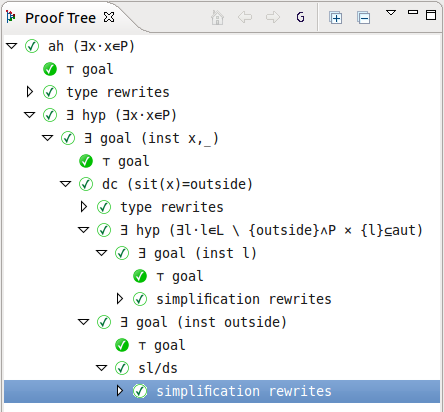
\includegraphics{img/tutorial/tut_10_proof_tree_final.png}
    \caption{Searching hypothesis for $outside$: The third one is \textsf{axm4}.}
    \label{fig_tut_10_final_proof_tree}
  \end{center}
\end{figure}



\subsection{Deadlock Freeness of First Refinement}
\label{tut_location_first_refinement}

Now we are going to explain the main complexity of our model: the deadlock freeness proof for the first refinement. 

\info{Please remember that post-tactics should still be disabled before starting this part of the tutorial.} 

The difference between the first refinement and the initial model is that a new constant \textsf{com} has been added in order to describe which rooms are connected. Additionally, we have a constant \textsf{exit}, which allows anybody to get outside.  Please consult the Event-B book (\ref{abrial_2010}) for the details regarding this model.

The event \textsf{INITIALISATION} does not change, but the event \textsf{PASS} is refined as a consequence. We assume that a person can move to another location $l$ if they have the authorisation to be in $l$ (already defined in the abstraction) and also if the location $l$ is connected to the location $p$ where the person is at this precise moment (represented by $sit(p)$).

\pencil{
\begin{description}
\nItemX{ grd12 }{ sit(p)\mapsto l \in  com }
\end{description}
}

As in the last section (\ref{tut_initial_model}), open the \texttt{door\_1} machine and add a derived invariant (theorem) called \textsf{DLF} as follows\footnote{In the future, it might be worthwhile to change this theorem to take care of a couple of issues. It only states that at least one person can move, and it may be better to state that every person can move.  Furthermore, this statement is unable to detect live locks\index{live lock}: A situation where the system oscillates between a small number of states.}: 

\pencil{
\begin{description}
	\nItemX{ DLF }{ \exists q, m \cdot (q \mapsto m \in aut \wedge sit(q) \mapsto m \in com)  }
\end{description}
}

Save the file. Once again, the prover fails to prove this theorem automatically. What we want to prove is that ``at least one person authorized to be in a location must also be authorized to go in another location which communicates with the first one''.

Switch over to the proving perspective and double click on \textsf{DLF/THM} to begin proving. When getting started, it is often a good idea to subdivide a proof into cases.  In this case, one distinction of cases should be to determine whether the person is outside or not.  

First we need a variable denoting a location in order to distinguish between the two cases. We use the deadlock freeness invariant from the initial model for this purpose. Search through the possible hypotheses and add this theorem to the selected hypotheses (Figure~\ref{tut_10_ref_proof1}).

\begin{figure}[!ht]
\begin{center}
	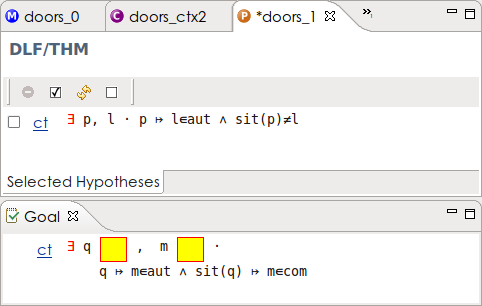
\includegraphics[]{img/tutorial/tut_10_ref_proof1.png}
	\caption{Adding a hypothesis to instantiate a variable for a case distinction.}
	\label{tut_10_ref_proof1}
\end{center}
\end{figure}

Now click on the red $\exists$ to instantiate the variables p and l. This will allow us to make the case distinction. To do this, we enter the following in the Proof Control View:

$$ sit(p) = outside $$

Now press the \icon{rodin/dc_prover.png} button.  This will create three new nodes in the proof tree: The first one is once again the well-definedness condition, followed by the two cases that we have just defined.  As always, use the \icon{rodin/auto_prover.png} button to verify the well-definedness condition.

The first case is dealing with $sit(p) = outside$.  To verify this case, we need to use\textsf{axm7}, which states that at least one authorized room is connected to the outside:

\pencil{
\begin{description}
	\nItemX{ axm7 }{ \exists l\qdot l\in L\setminus \{ outside\}  \land  outside\mapsto l\in com \land  P\cprod \{ l\} \subseteq aut  }
\end{description}
}

Add \textsf{axm7} to the list of hypotheses.  We would like to work with an instance of a location, so we instantiate this hypothesis by clicking on its red $\exists$ symbol.

\info{Note that Rodin instantiated the variable with the name $l0$ instead of $l$ because the name $l$ already exists from the previous instantiation.}

Now we have variables to instantiate our goal as well.  We enter the value $p$ in the yellow box for q and $l0$ in the yellow box for m (figure~\ref{tut_10_ref_proof2}) and press the red  $\exists$.

\begin{figure}[!ht]
\begin{center}
	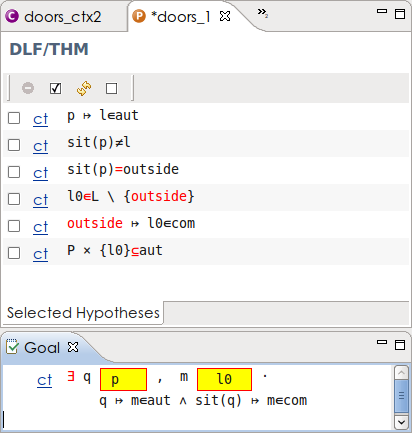
\includegraphics[]{img/tutorial/tut_10_ref_proof2.png}
	\caption{Preparing the instantiation by providing values for $p$ and $l0$.}
	\label{tut_10_ref_proof2}
\end{center}
\end{figure}

This results in two new nodes to the proof tree, the first one being the well-defined proof obligation.  The last remaining proof obligation can be solved with the given hypotheses.  Clicking \icon{rodin/p0.png} will discharge both of these proof obligations.

Now the first case is resolved.  Now let's consider the second case, $sit(p) \neq outside$.  We would like to instantiate the quantifier again, but this time we have to use different values.  We still have p to substitute for q, but for the location we use the exit relationship: Our axioms tell us that there is always an exit from every location, so $exit(sit(p))$ should be a valid substitution for m. Let's perform the substitution.  This advances our proof tree with a new node (and the well-definedness proof obligation, which we discharge with one click).

The resulting proof obligation is a conjunction.  We can discharge the two parts of it by clicking on the red $\land$ symbol in the goal view. This results in two simpler goals in the proof tree.  We start with the \textbf{second} goal.

\info{We start with the second goal instead of the first goal because doing so will provide us with hypotheses that will be beneficial in discharging the first goal.  How do we know this? By experience and by playing with the proofs for a long time.  Depressingly, there is no easy rule to guide us through the proving process. There are just general guidelines and experience.}

The goal we start with is:

$$ sit(p) \mapsto exit(sit(p)) \in com $$

None the hypotheses that we have added so far contain $com$, so add \textsf{axm4} to the selected hypotheses:

\pencil{
\begin{description}
\nItemX{ axm4 }{ exit \subseteq  com }
\end{description}
}

Hit the \icon{rodin/p0.png} button, and Rodin discharges the goal.

Now deal with the last undischarged goal:

$$ p \mapsto exit(sit(p)) \in aut $$

This statement means that the person is authorized to follow the exit. To discharge this proof obligation we need to use \textsf{axm6}, which essentially states that ``Everybody has the permission to leave from wherever they are'':

\pencil{
\begin{description}
\nItemX{ axm6 }{ aut \ransub  \{ outside\}  \subseteq  (aut ; exit^{-1} )  }
\end{description}
}

Remove the inclusion by clicking on the red $\subseteq$, which results in a hypothesis with universal quantifier. Instantiate this with the variables that we already have on hand.  Instantiate x with p and x0 with sit(p).  Examine this formula and try to understand what it means.

This results in two more goals in our proof tree. The first goal is the well-definedness condition which we discharge with the \icon{rodin/auto_prover.png} button.

The remaining goal is simple and essentially states that following the current position along the exit route will lead to a location where the user is authorized:

$$ p \subseteq exit(sit(p)) \in aut $$

We cannot discharge this with the \icon{rodin/p0.png} prover; However, using the \icon{rodin/p1.png} prover will discharge it.  Using \icon{rodin/p1.png} is the same as selecting related hypotheses with \icon{rodin/lasoo_prover.png} and then using \icon{rodin/p0.png}.  The danger of this approach is that if too many hypotheses are added, the prover may not be able to find a solution before timing out.  In this case, it worked.

\info{As an exercise, try to manually identify the hypotheses that were required to discharge this goal.}


This concludes this section of the tutorial. Be aware that we have just looked at one small aspect of a rather sophisticated model.  Also, please be aware that this tutorial gave you only an introduction to proving.  To become an expert, we encourage you to study interesting models and to practice.

%%% Local Variables: 
%%% mode: latex
%%% TeX-master: "rodin-doc"
%%% End: 
